\newpage
\subsection{Empty Rectangle}
Für die Technik \textit{Empty Rectangle} gilt das selbe wie für alle \textit{Single Digit Patterns}, es wird nur eine Ziffer betrachtet und der Name leitet sich aus der Form der Anordnung der Ziffern ab. Um ein \textit{Empty Rectangle} zu finden, wird ein Block gesucht, in dem ein Kandidat ausschließlich noch in einer Zeile und in einer Spalte vorkommen kann. Dann bilden die verbliebenen Kandidaten eine Ecke eines \textit{Empty Rectangles}.

\begin{figure}[h]
\begin{center}
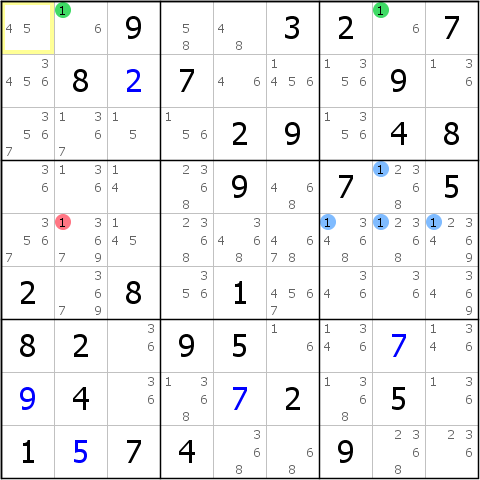
\includegraphics{./img/empty_rectangle.png}
\caption{Empty Rectangle}
\end{center}
\end{figure}

In \textbf{Abbildung 3.12} sehen wir ein \textit{Empty Rectangle}, das von Block 5 ausgeht. Die verbleibenden Kandidaten der Ziffer 1 können hier nur noch in Zeile 4 und Spalte 5 stehen. Wenn wir Zeile 7 betrachten, dann sehen wir, dass die Ziffer 1 hier nur noch an zwei Positionen stehen kann, nämlich an der fünften und an der neuten. Wir betrachten nun diese beiden Fälle getrennt. Wenn die Ziffer 1 in z7s9 steht, dann ist die Ziffer 1 in z4s9 direkt ausgeschlossen. Wenn sie in z7s5 steht, dann kann sie in Block 5 nur noch an einer Position stehen, nämlich z4s6. Auch in diesem Fall ist die Ziffer 1 dann im Feld z4s9 ausgeschlossen. Daher kann sie dort als Kandidat gelöscht werden.